% !TeX spellcheck = en_US
\chapter{Applications}
\label{chap:Applications}


\lettrine[lines=4,slope=0.6em,findent=-1em]{\color{BrickRed}A}{s} the name said, the Quadratic Assignment Problem was firstly studied to solve the  problem involving  assignment of $n$ facilities to $n$ locations. Nevertheless. QAP appears in several seemingly unrelated decision problems such as keyboard design~\cite{Burkard1977}, scheduling~\cite{Geoffrion1976}, arrangements of micro array chips~\cite{CarvalhoJr2006}, numerical analysis~\cite{Brusco2000}, forest park management~\cite{Bos1993}, Traveling Salesman Problem (TSP)~\cite{Sahni_1976,Cela1998} and so on. In this chapter we describe some of these applications; many others can be found on~\cite{Burkard2012}.

\section{Hospital Layout}
\label{sec:Hospital Layout}
In 1975 the Ahmed Mahe Hospital of Cairo (Egypt) was composed by six major departments. One of them (the Outpatient) is formed by $19$ clinics, listed in table~\ref{tab:Elshafei}.

\begin{table}%[htp]
%	\footnotesize
\centering
\caption{Facilities of Outpatient department.}
\label{tab:Elshafei}
\begin{tabular}{*2{cl}}
	\toprule
Facility & Clinic & Facility & Clinic \\
\midrule	
1 & Receiving and Recording& 11 & X-Ray \\
2 & General Practitioner & 12 & Orthopedic\\
3 & Pharmacy & 13 & Psychiatric \\
4 &Gynecological \& Obstetric & 14 & Squint \\
5 & Medicine& 15 & Minor Operations \\
6 & Pediatric & 16 & Minor Operations\\
7 & Surgery & 17 & Dental\\
8 & Ear, Nose \& Throat & 18 & Dental Surgery\\
9 & Urology & 19 & Dental Prosthetic\\
10 & Laboratory & &  \\ 
\bottomrule

\end{tabular}	
\end{table}

 The problem was to find the optimal layout of the department minimizing the total distance traveled by patients. Alwalid Elshafei~\cite{Elshafei_1977} modeled this  as a QAP. This problem has dimension $n=19$. 


The problem is symmetric, since every patient must return to the first clinic he visited to mark off his card. 

The distance matrix $\bm D= (d_{ij})$ contains the distances between the clinics $i$ and $j$.
The flow matrix $\bm F= (f_{ij})$ contains flows between clinics $r$ and $s$ on a yearly basis. 

The highest flow is $76687$: between Receiving and Recording and General Practitioner. The second one ($40951$) is between General Practitioner and Pharmacy. The third one ($13732$) is between Receiving and Recording and Dental clinic. Moreover, the flow between facilities 15 and 16 was set $99999$, to force them to be in two adjacent locations in the final solution.

The distances between locations were measured by tracing the paths taken by patients while moving from a clinic to another. Whenever the movement involved a change in floors, the corresponding vertical distance was multiplied by $3$~\cite{Elshafei_1977}.


Elshafei and Bazaraa eliminated nearly $20\%$ of unnecessary traffic by patients, resulting in an overall more effective treatment center. As a result, their findings were implemented in a new layout of the department~\cite{Elshafei_1977}.

In 1978 Krarup~\cite{Krarup1978} described a related problem for Regensburg Clinic, in Germany. In 2015 Feng and Su~\cite{Feng2015} applied this model to the Tongji hospital, Shanghai (China), reducing the average walking time for the outpatients by \num{11.55}\%. In 2016 Helbert et al~\cite{Helber2015} followed a similar approach for Hannover Medical School, Germany.

\section{Wedding banquet}
\label{sec:Wedding_banquet}

In 1970 Muller~\cite{MuellerMerbach1970} described the following situations: we want to arrange $n$  wedding guests around a table minimizing the \textit{annoyance} between them or, if we prefer, maximizing the total pleasantness. 

We know the distances $d_{ij}$ between seat $i$ and $j$. We can consider any form of tables (rectangular, round, \dots) or sets of tables. The only thing that matters is knowing the relative distance between seats.



\noindent As regards guests, we consider the intensity of relationship $f_{rs}$ between every guest $r$ and $s$. High values of $f_{rs}$ correspond to a good relationship. 
\begin{wrapfloat}{figure}{i}{0pt}
	\vspace{-10pt}
	\includegraphics[width=.20\textwidth]{Wedding_table}
	\vspace{-10pt}	
\end{wrapfloat}The value of $f_{rs}$ can be related to several characteristics: age, relationship status, interest groups, degrees of acquaintance, sympathy. For example, the author (which has not yet organized any wedding) thinks that kids should be placed together, and near their parents. Note that the spouses should know how good the relationships between guests are. Finally, note that in general $f_{rs}\neq f_{sr}$.

 
The wedding banquet problem can be described as follows:

\begin{equation}
\min_{\pi \in \Sn} \left[\sum_{i=1}^n\sum_{j=1}^n f_{ij}d_{\pi(i)\pi(j)}\right].
\end{equation}

\noindent As we can see, this is the  combinatorial form of the QAP.

\section{Backboard wiring}
\label{sec:BackboardWiring} 

This problem was studied by Leon Steinberg in 1961~\cite{Steinberg1961}. 

The goal of this problem is to minimize the length of connections between units that have to be placed on a rectangular grid, as shown in figure~\ref{fig:Steinberg}. The dimension of the problem is $n=36$.

\begin{figure}[htp]
\centering

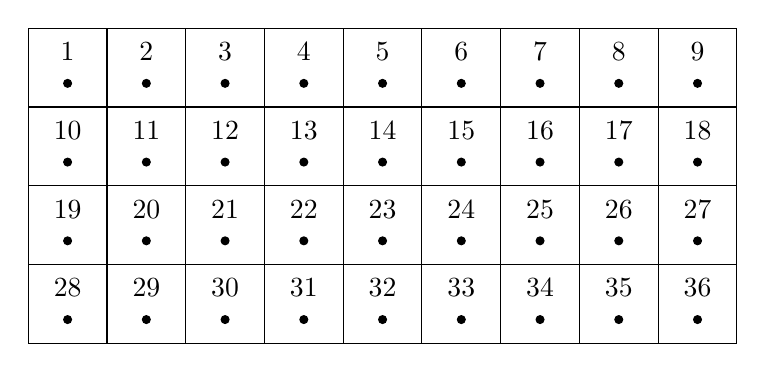
\begin{tikzpicture}
\draw (0,0) grid (9,4) ;
 \node at (           0.5,           3.7) {           1} ;
\node at (           1.5,           3.7) {           2} ;
\node at (           2.5,           3.7) {           3} ;
\node at (           3.5,           3.7) {           4} ;
\node at (           4.5,           3.7) {           5} ;
\node at (           5.5,           3.7) {           6} ;
\node at (           6.5,           3.7) {           7} ;
\node at (           7.5,           3.7) {           8} ;
\node at (           8.5,           3.7) {           9} ;
 \node at (           0.5,           2.7) {          10} ;
\node at (           1.5,           2.7) {          11} ;
\node at (           2.5,           2.7) {          12} ;
\node at (           3.5,           2.7) {          13} ;
\node at (           4.5,           2.7) {          14} ;
\node at (           5.5,           2.7) {          15} ;
\node at (           6.5,           2.7) {          16} ;
\node at (           7.5,           2.7) {          17} ;
\node at (           8.5,           2.7) {          18} ;
 \node at (           0.5,           1.7) {          19} ;
\node at (           1.5,           1.7) {          20} ;
\node at (           2.5,           1.7) {          21} ;
\node at (           3.5,           1.7) {          22} ;
\node at (           4.5,           1.7) {          23} ;
\node at (           5.5,           1.7) {          24} ;
\node at (           6.5,           1.7) {          25} ;
\node at (           7.5,           1.7) {          26} ;
\node at (           8.5,           1.7) {          27} ;
 \node at (           0.5,           0.7) {          28} ;
\node at (           1.5,           0.7) {          29} ;
\node at (           2.5,           0.7) {          30} ;
\node at (           3.5,           0.7) {          31} ;
\node at (           4.5,           0.7) {          32} ;
\node at (           5.5,           0.7) {          33} ;
\node at (           6.5,           0.7) {          34} ;
\node at (           7.5,           0.7) {          35} ;
\node at (           8.5,           0.7) {          36} ;
 \draw[fill=black] (           0.5,           0.3) circle (0.05cm) ;
\draw[fill=black] (           1.5,           0.3) circle (0.05cm) ;
\draw[fill=black] (           2.5,           0.3) circle (0.05cm) ;
\draw[fill=black] (           3.5,           0.3) circle (0.05cm) ;
\draw[fill=black] (           4.5,           0.3) circle (0.05cm) ;
\draw[fill=black] (           5.5,           0.3) circle (0.05cm) ;
\draw[fill=black] (           6.5,           0.3) circle (0.05cm) ;
\draw[fill=black] (           7.5,           0.3) circle (0.05cm) ;
\draw[fill=black] (           8.5,           0.3) circle (0.05cm) ;
\draw[fill=black] (           0.5,           1.3) circle (0.05cm) ;
\draw[fill=black] (           1.5,           1.3) circle (0.05cm) ;
\draw[fill=black] (           2.5,           1.3) circle (0.05cm) ;
\draw[fill=black] (           3.5,           1.3) circle (0.05cm) ;
\draw[fill=black] (           4.5,           1.3) circle (0.05cm) ;
\draw[fill=black] (           5.5,           1.3) circle (0.05cm) ;
\draw[fill=black] (           6.5,           1.3) circle (0.05cm) ;
\draw[fill=black] (           7.5,           1.3) circle (0.05cm) ;
\draw[fill=black] (           8.5,           1.3) circle (0.05cm) ;
\draw[fill=black] (           0.5,           2.3) circle (0.05cm) ;
\draw[fill=black] (           1.5,           2.3) circle (0.05cm) ;
\draw[fill=black] (           2.5,           2.3) circle (0.05cm) ;
\draw[fill=black] (           3.5,           2.3) circle (0.05cm) ;
\draw[fill=black] (           4.5,           2.3) circle (0.05cm) ;
\draw[fill=black] (           5.5,           2.3) circle (0.05cm) ;
\draw[fill=black] (           6.5,           2.3) circle (0.05cm) ;
\draw[fill=black] (           7.5,           2.3) circle (0.05cm) ;
\draw[fill=black] (           8.5,           2.3) circle (0.05cm) ;
\draw[fill=black] (           0.5,           3.3) circle (0.05cm) ;
\draw[fill=black] (           1.5,           3.3) circle (0.05cm) ;
\draw[fill=black] (           2.5,           3.3) circle (0.05cm) ;
\draw[fill=black] (           3.5,           3.3) circle (0.05cm) ;
\draw[fill=black] (           4.5,           3.3) circle (0.05cm) ;
\draw[fill=black] (           5.5,           3.3) circle (0.05cm) ;
\draw[fill=black] (           6.5,           3.3) circle (0.05cm) ;
\draw[fill=black] (           7.5,           3.3) circle (0.05cm) ;
\draw[fill=black] (           8.5,           3.3) circle (0.05cm) ;
\end{tikzpicture}
\caption{Backboard of Steinberg's problem.}
\label{fig:Steinberg}
\end{figure}


\noindent As  an example, consider two points $\mathsf P_i=(x_i,y_i)$ and $\mathsf P_j=(x_j,y_j)$. We can refer to their distance $d_{ij}=\mathrm{d}\left(\mathsf P_i,\mathsf P_j\right)$ in (at least) three different ways:

\begin{enumerate}
	\item[a)] Manhattan distance (or $1$-norm): in this case \[d^\mathrm{a}_{ij}=\abs{x_i-x_j}+\abs{y_i-y_j}.\]
	\item[b)] Squared Euclidean distance: \[d^\mathrm{b}_{ij}=\left(x_i-x_j\right)^2+\left(y_i-y_j\right)^2.\]
	\item[c)] Euclidean distance multiplied by $1000$: \[d^\mathrm{c}_{ij}=\num{1000}\cdot \sqrt{\left(x_i-x_j\right)^2+\left(y_i-y_j\right)^2}.\]
\end{enumerate}

The distance matrix $\bm D=(d_{ij})$ contains the distance between each pair of positions, depending on the distance considered.


 The flow matrix  $\bm F=(f_{rs})$ (the same for all the three distances) provides the number of connections to make between the units $r$ and $s$. 
 
 The goal is to minimize the total length of wire used to interconnect the components.
 

\section{Keyboard design}
\label{sec:Keyboard}

This problem was firstly studied by Burkard and Offerman in 1977~\cite{Burkard1977}.

The goal is to find out what would be, in theory, the best typewriter keyboards for various languages and for mechanical or electrical machines. 

Since the number of letters on \textsc{ISO} basic Latin alphabet is $26$, the size of this problems is  $n = 26$. 

The distance matrix $\bm D$ corresponds to the time between
the typing of two keys (the time depends on the fact that the machine is an electrical or a
mechanical one).

The flow matrix $\bm F$ contains the frequencies of appearance of two letters in a given language~\cite{Taillard1995}.

As four different languages and two typewriters are considered, there
are eight problems of this type. 



English, French, German and Dutch languages are considered in literature~\cite{Taillard1995}. 
The proposed methods yield improvements
of $7$-$10\%$ compared with the international standard keyboard.

In 2009  Dell'Amico et al~\cite{DellAmico2009} studied the problem of designing a single-finger keyboard for smartphones.


%\newpage
\section{Dartboard design}
\label{sec:Darboard}
The game of darts consists in hitting sectors of a circular target (called \textit{dartboard}) with darts in order to obtain the greatest possible score. 

\begin{wrapfloat}{figure}{I}{0pt}
	\vspace{-10pt}	
	\centering
	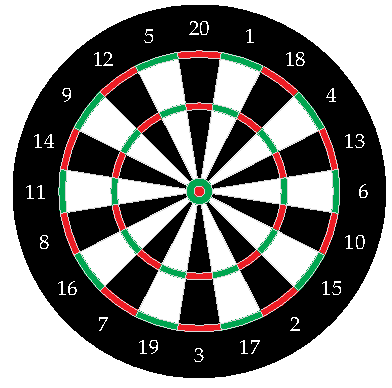
\includegraphics[width=.40\textwidth]{dartboard}
	\caption{A dartboard.}
	\label{fig:Dartboard}
	\vspace{-10pt}		
\end{wrapfloat}
 Let us focus on the numbers around the dartboard,  shown in figure~\ref{fig:Dartboard}. As we can see, there are $20$ numbers (from $1$ to $20$), each one corresponding to a sector of the dartboard. Why  these specific numbers were  chosen? If we look at the number $20$ (the biggest one) we can see that its closest numbers are $1$ and $5$. Hence, aiming the sector with $20$ has a great risk, since doing a mistake results in loosing many points.
This implies a maximization problem: choosing the numbers around a dartboard to maximize the risk. 


The current scoring system
was devised in 1896 by Brian Gamlin values~\cite{Eiselt1991}. In 1991 Eiselt and Laporte~\cite{Eiselt1991} described this problem as an instance of QAP. 

 Let $\pi(k)$ denote the number placed in position $k$ on the dartboard (starting from an arbitrary position) and let $\pi = [\pi(1), \dots , \pi(20)]$ be any permutation of the numbers $1,\dots , 20$.  In the following lines,  $\pi(k)$ must be interpreted as $\pi(k \mod 20)$ whenever $k < 1$ or $k > 20$.

 Now, consider a player aiming at $\pi(k)$. Let us suppose that he hits $\pi(k)$ with probability $p_0$, $\pi(k \pm 1)$ with probability $p_1$ and, in general,  $\pi(k\pm t)$ with probability $p_t$ ($t=0,\dots,10$). Since $p_t$ are probabilities, it must be 
\begin{equation}
	\label{eq:dart}
p_0  +2\sum_{t=1}^9 p_t+p_{10}=1.
\end{equation}
As suggested by Eiselt and Laporte~\cite{Eiselt1991}, it seems realistic enough to
restrict ourselves to the case where players never hit more than two sectors away from their target. Therefore, we assume  that $p_t=0$ for $t > 2$. 

Thus, equation~\eqref{eq:dart} implies
\begin{equation}
p_0 = 1 - 2 p_1 -2 p_2.
\end{equation}

\noindent Moreover, we may assume $p_2= \theta p_1$ with $\theta \in (0,1)$.

Hence, for every $k \in \{1,\dots,20\}$, the expected deviation from the aimed score is


\scriptsize
\begin{align}
	\label{eq:Dartboard2}
	\notag 
		&\quad \  p_1 \Big( \abs*{\pi(k+1)-\pi(k)}+ \abs*{\pi(k-1)-\pi(k)} \Big)
		+ \theta p_1 \Big(\abs*{\pi(k+2)-\pi(k)} + \abs*{\pi(k-2)-\pi(k)}\Big)\\
&=p_1 \bigg[ \Big( \abs*{\pi(k+1)-\pi(k)}+ \abs*{\pi(k-1)-\pi(k)} \Big)
+ \theta \Big(\abs*{\pi(k+2)-\pi(k)} + \abs*{\pi(k-2)-\pi(k)}\Big)\bigg]		
\end{align}
\normalsize
Notice that in~\eqref{eq:Dartboard2}  the probability $p_1$ is constant and, if we sum for $k$, every term is counted twice.

 Therefore, the objective function $z$ to be maximized is 

\begin{equation}
	\label{eq:Dart_z}
z = \sum_{k=1}^{20} \abs*{\pi(k+1)-\pi(k)} + \theta \sum_{k=1}^{20} \abs*{\pi(k+2)-\pi(k)}.
\end{equation}


\noindent Now, fix a permutation $\pi \in S_{20}$. This problem has an equivalent binary programming form. For every $i,j \in \{1,\dots,20\}$, define the binary variables $x_{ij}$ as equal to $1$ if (in the permutation $\pi$) $i$ is followed immediately by~$j$ (i.e. if $\pi(k) = i$ and $\pi(k + 1) = j$ for some $k$), and equal to $0$ otherwise. In practice, 
\begin{equation}
x_{ij}= \begin{cases}
	1 & \text{if exists $k$ such that $\pi(k)=i$ and $\pi(k+1)=j$;} \\
	0 & \text{otherwise.}
\end{cases}
\end{equation}

\noindent First, we note that $\bm X=(x_{ij})$ is a permutation matrix. Secondly, for $i,j\in\{1,\dots,n\}$ it follows that 
\small
\begin{equation}
	\label{eq:Dart_lineare}
\begin{split}	
\abs{i-j} \ x_{ij}\neq 0 
&\iff \text{$\exists k$ such that  $i=\pi(k)$ and $j=\pi(k+1)$}\\
&\iff \abs{i-j} \ x_{ij} = \abs*{\pi(k+1)-\pi(k)}	.
\end{split}	
\end{equation}	
\normalsize



Now, similar to~\eqref{eq:Dart_lineare}, for $i,j,l\in \{1,\dots,n\}$, we get
\small
\begin{equation}
	\label{eq:Dart_Quadratica}
\begin{split}	
	\abs{i-l} \ x_{ij} \, x_{jl}\neq 0 
	&\iff \text{$\exists k$ such that  $i=\pi(k)$, $j=\pi(k+1)$ and $l=\pi(k+2)$}\\
	&\iff \abs{i-l} \ x_{ij} \, x_{jl} = \abs*{\pi(k+2)-\pi(k)}	.
\end{split}	
\end{equation}
\normalsize


Therefore, summing each terms on~\eqref{eq:Dart_lineare} and~\eqref{eq:Dart_Quadratica}, the objective function in~\eqref{eq:Dart_z} can be rewritten:

\begin{gather}
z =	\sum_{i=1}^{20}\sum_{j=1}^{20}\abs{i-j} \ x_{ij} +\theta\sum_{i=1}^{20}\sum_{j=1}^{20}\sum_{l=1}^{20}\abs{i-l} \ x_{ij}\, x_{jl}.
\end{gather}

\noindent Finally, the problem can be written in the following form:

\begin{equation}
	\begin{split}
&\max \left[ \sum_{i=1}^{20}\sum_{j=1}^{20} \abs{i-j} \  x_{ij} + \sum_{i=1}^{20}\sum_{j=1}^{20}\sum_{l=1}^{20} \abs{i-l} \theta  \, x_{ij}\,x_{jl}\right]\\
&\text{ s.t} \quad  \sum_{i=1}^n x_{ij} = 1 \qquad \forall j\in\{1,\dots,n\}\\
&\phantom{\text{ s.a}} \quad   \sum_{j=1}^n x_{ij} = 1 \qquad \forall i\in \{1,\dots,n \} \\
&\phantom{\text{ s.a}} \quad  x_{ij}\in \{0,1\} \qquad \forall i,j \in \{1,\dots,n \}  \\
\end{split}
\end{equation}


Which can be expressed as a QAP instance (see~\cite[p. 116]{Eiselt1991}).
